\documentclass[a4paper, 11pt, twoside]{book}
\usepackage[style=numeric]{biblatex}
\usepackage{tbagrelstandard}
\usepackage{concretefull}
\usepackage{float}
\usepackage{pdfpages}

\DeclareFontShape{T1}{lmss}{sbc}{sc}{<->ssub * lmss/sbc/n}{}

\RequirePackage{color, xcolor}
\RequirePackage{listings}
\lstset{
  basicstyle=\ttfamily\normalsize\color{black!90},
  stringstyle=\color{black!70},
  commentstyle=\itshape\color{black!60},
  identifierstyle=\color{black!90},
  keywordstyle=\color{black!100}\bfseries,
  numberstyle=\ttfamily\small\color{black!50},
  numbers=left,
  numbersep=10pt,
  backgroundcolor=\color{black!1},
  rulecolor=\color{black!30},
  title=\large\ttfamily\lstname,
  breakatwhitespace=true,
  breaklines=false,
  captionpos=b,
  frame=single,
  keepspaces=true,
  showspaces=false,
  showstringspaces=false,
  showtabs=false,
  stepnumber=1,
  tabsize=4,
  numberblanklines=true,
  frameround=tttt,
}

\tabularnewline

\bibliography{bibliography}

\DeclareFieldFormat*{title}{{\itshape #1}}
\DeclareFieldFormat*{note}{#1}
% \DeclareFieldFormat*{usera}{\tt{#1}}

% \renewbibmacro*{url}{\hreff{\printfield{url}}{\printfield{usera}}}

\DeclareBibliographyDriver{online}{%
  \usebibmacro{bibindex}%
  \usebibmacro{begentry}%
  \printfield{title}\\%
  \printfield{note}\quad%
  {\footnotesize%
  \usebibmacro{urldate}%
  }
}

% \DeclareFieldFormat{url}{}
% \DeclareFieldFormat{usera}{#1}
% \AtEveryBibitem{%
%     \csappto{blx@bbx@\thefield{entrytype}}{% put at end of entry
%         \iffieldundef{usera}{%
%           \space \textbf{No annotation!}}{%
%           \space\printfield{usera}
%         }
%     }
% }

\newcommand{\hreff}[2]{\href{#1}{\tt{#2}}}

\edef\restoreparindent{\parindent=\the\parindent\relax}
\usepackage{parskip}
\restoreparindent

\geometry{inner=3cm,outer=2cm,top=2.5cm,bottom=2cm}

\AtBeginDocument{\addtocontents{toc}{\protect\thispagestyle{plain}}}
%\patchcmd{\chapter}{\thispagestyle{plain}}{}{}{}
\patchcmd{\bibliography}{\thispagestyle{empty}}{\thispagestyle{plain}}{}{}

\makeatletter
\def\cleardoublepage{\clearpage\if@twoside \ifodd\c@page\else
\thispagestyle{empty}%
\hbox{}\newpage\thispagestyle{empty}\if@twocolumn\hbox{}\newpage\thispagestyle{empty}\fi\fi\fi}
\renewcommand\part{%
  \if@openright
    \cleardoubelpage
  \else
    \clearpage
  \fi
  \thispagestyle{empty}%
  \if@twocolumn
    \onecolumn
    \@tempswatrue
  \else
    \@tempswafalse
  \fi
  \null\vfil
  \secdef\@part\@spart}
\def\@endpart{\if@twoside
               \if@openright
               \fi
              \fi
              \if@tempswa
                \twocolumn
              \fi}

\def\cleardoubelpage{\clearpage
 \if@twoside
  \ifodd\c@page
   \null\thispagestyle{empty}\newpage\thispagestyle{empty}
   \if@twocolumn\null\newpage\thispagestyle{empty}\fi
   \else\fi
  \fi
 }%
 \makeatother

\renewcommand\lstlistlistingname{Table des listings}

\newcommand{\HRule}{\rule{\linewidth}{0.5mm}}
\newcommand{\anglais}[1]{\it{#1}}
\newcommand{\tech}[1]{\sf{#1}}
\newcommand{\env}[1]{\sf{#1}}
\newcommand{\placeholder}[1]{\,$\langle\,\text{\textnormal{#1}}\,\rangle$\,}

\renewcommand{\tn}{TELECOM Nancy}
\newcommand{\fisa}{\sc{fisa}}

\let\citeoriginal\cite
\renewcommand{\cite}[1]{\textsuperscript{\citeoriginal{#1}}}

\let\paragraphoriginal\paragraph
\renewcommand{\paragraph}[1]{\paragraphoriginal{#1}\mbox{}}

\renewcommand{\headrulewidth}{0.5pt}
\renewcommand{\footrulewidth}{0pt}

\makeindex

\begin{document}
\frontmatter
\pagestyle{empty}

%------------------------------------------------------------------------------
% https://fr.overleaf.com/latex/examples/title-page-with-logo/hrskypjpkrpd
\begin{titlepage}

\center{}

%------------------------------------------------------------------------------
% HEADING SECTIONS
%------------------------------------------------------------------------------

\hspace{0pt}
\vfill{}

\textsc{\large \tn{}}\\[1.2cm]

%------------------------------------------------------------------------------
% TITLE SECTION
%------------------------------------------------------------------------------

\HRule \\[0.4cm]
{ \huge \bfseries Rapport de projet PPII (FISA)}\\
\HRule \\[1.5cm]

%------------------------------------------------------------------------------
% AUTHOR SECTION
%------------------------------------------------------------------------------

\begin{minipage}{0.38\textwidth}
\begin{flushleft} \large
\emph{Auteurs~:}\\
Thomas~\textsc{Bagrel}
\end{flushleft}
\end{minipage}
\hfill
\begin{minipage}{0.58\textwidth}
\begin{flushright}
\begin{tabular}{lr}
\mbox{}\\
Timothée~\textsc{Adam}
\end{tabular}
\end{flushright}
\end{minipage}\\[1.5cm]

%------------------------------------------------------------------------------
% DATE SECTION
%------------------------------------------------------------------------------

{\large Année 2018 - 2019}\\[1.2cm]

%------------------------------------------------------------------------------
% LOGO SECTION
%------------------------------------------------------------------------------


\includegraphics[height=2.5cm]{resources/logo_tn.jpg}\\[1cm]

\vfill{}
\end{titlepage}
\clearpage{}

%------------------------------------------------------------------------------

% page blanche (2ème de couverture)
~\vfill
\clearpage{}

%------------------------------------------------------------------------------

\pagestyle{plain}
\section*{Déclaration sur l'honneur de non-plagiat}
\addcontentsline{toc}{section}{Déclaration sur l'honneur de non-plagiat}

Nous soussignons Thomas \sc{Bagrel} et Timothée \sc{Adam}, élèves de 1\tss{ère} année \fisa{} à \tn{}, déclarons nous être s sur les différentes formes de plagiat existantes et sur les techniques et normes de citation et référence.

Nous déclarons en outre que le travail rendu est un travail original, issu de notre réflexion personnelle, et qu'il a été rédigé entièrement par nos soins. Nous affirmons n'avoir ni contrefait, ni falsifié, ni copié tout ou partie de l'\oe{}uvre d'autrui, en particulier texte ou code informatique, dans le but de nous l'accaparer.

Nous certifions donc que toutes formulations, idées, recherches, raisonnements, analyses, programmes, schémas ou autre créations, figurant dans le document et empruntés à un tiers, sont clairement signalés comme tels, selon les usages en vigueur.

Nous sommes conscients que le fait de ne pas citer une source ou de ne pas la citer clairement et complètement est constitutif de plagiat, que le plagiat est considéré comme une faute grave au sein de l'Université, et qu'en cas de manquement aux règles en la matière, nous encourrons des poursuites non seulement devant la commission de discipline de l'établissement mais également devant les tribunaux de la République Fran\c{c}aise.

\vfill{}

\hspace{7cm}\begin{minipage}{7cm}
\bf{Fait à Vand\oe{}uvre-lès-Nancy, le 2 juin 2019}

\vspace{2cm}

\phantom{<signature>}
\end{minipage}
\clearpage{}

%------------------------------------------------------------------------------

\section*{Avant-propos}
\addcontentsline{toc}{section}{Avant-propos}

Ce rapport relate les démarches et le travail que Thomas BAGREL et Timothée ADAM ont effectué sur le projet  \tt{ppii-2k19}. Il met en avant le contexte original et complexe dans lequel nous avons travaillé et les moyens que nous avons mis en place pour y faire face.

Les annexes disponibles à la fin du document constituent un complément d'information sur la phase de conception réalisée pour la partie base de données.

\hspace{3cm}

%------------------------------------------------------------------------------

\tableofcontents{}
\addcontentsline{toc}{section}{Table des matières}
\newpage\hbox{}\thispagestyle{empty}\cleardoublepage{}

%------------------------------------------------------------------------------
\mainmatter
\pagestyle{fancy}
\fancyhf{}

% \renewcommand*{\chaptermark}[1]{%
%   \def\delayedchaptermark{%
%     \bfseries%
%     \ifnum\value{chapter}>0 %
%       \chaptername~\thechapter.~%
%     \fi%
%     #1%
%   }
% }
\renewcommand*{\chaptermark}[1]{%
  \markboth{%
    \bfseries%
    \ifnum\value{chapter}>0 %
      \chaptername~\thechapter.~%
    \fi%
    #1%
  }{}
}
\renewcommand*{\sectionmark}[1]{%
  \markright{%
    \ifnum\value{chapter}>0 \ifnum\value{section}>0 %
      \thesection.~%
    \fi\fi
    #1%
  }%
}%

%\lhead[\expandafter\delayedchaptermark]{}
\lhead[\leftmark]{}
\chead{}
\rhead[]{\rightmark}

\lfoot{}
\cfoot{\thepage}
\rfoot{}

%-----------------------------------------------------------------------------%------------------------------------------------------------------------------%------------------------------------------------------------------------------

\chapter*{Introduction}
\chaptermark{Introduction}
\addcontentsline{toc}{chapter}{Introduction}
\addtocontents{toc}{\protect\vspace{-0.3cm}}

Ce projet de première année en apprentissage nous proposait de nous confronter à un sujet pluridisciplinaire mettant en jeu de nombreuses connaissances techniques et compétences afin de proposer un livrable de type ingénieur.

Nous allons donc présenter comment, dans la limite de nos connaissances et du temps dont nous disposions, nous avons aboutit à la réalisation d'une solution raisonnablement fonctionnelle respectant le plus de consignes initiales possibles.

Néanmoins, cette dernière est loin d'être parfaite (en particulier, l'éventuelle partie 3 n'est pas encore traitée), et nous ne manquerons donc pas d'expliquer dans la dernière partie de ce rapport les nombreuses difficultés auquelles nous avons été confrontées.

Nous tenterons de détailler au mieux les raisons ayant motivé les différents choix que nous avons été obligés de faire pour réaliser ce projet, ainsi que les points sur lesquels plusieurs solutions étaient possibles.

\chapter{Organisation du travail}
\section{Une communication assidue}

Afin de réaliser ce projet, nous nous sommes immédiatement mis d'accord sur le fait qu'une communication importante était déterminante pour la réussite de ce dernier.

Ainsi, nous organisions régulièrement des \emph{stand-up meetings} pendant les temps de pause afin de fixer les objectifs des différents membres du groupe pour les jours à venir, ainsi que pour planifier certaines périodes de travail communes.

De plus, une communication par l'intermédiaire de \sf{Discord} nous permettait de partager rapidement questions, réponses, propositions diverses et fragments de code.

Cette méthode s'est révélée assez efficace tout au long du projet, même s'il nous arrivait par moment d'oublier les \emph{stand-up meetings} prévus, entraînant un léger retard dans l'organisation du projet.

\section{Distribution du travail}

Les attendus importants de la part des enseignants pour ce projet, sa difficulté technique ainsi que le peu de temps disponible pour réaliser ce dernier nous ont poussé à mettre en place une distribution du travail basée sur le gain de temps et la productivité.

Si cela a impliqué que les personnes les plus à l'aise avec le \sf{C} gèrent majoritairement le \sf{C} (de même que pour le \sf{SQL}), cette technique nous a permis de progresser rapidement dans le projet dans les moments difficiles.

De plus, cela a également permis aux membres du groupe moins à l'aise avec une technologie de réaliser une véritable montée en compétences sur cette dernière, au travers des revues de code, de l'inspection mutuelle du code, ainsi que des nombreuses questions posées à l'occasion des \emph{meetings} journaliers ou encore des réunions de chantier.

\newpage
\section{Conventions}

Pour gérer au mieux ce projet contenant une part non négligeable de développement logiciel, nous avons choisi de poser des contraintes assez importantes sur le style de code à adopter ainsi que sur le choix des noms de variables, classes\ldots{}

Nous pensons que cela a été très bénéfique, puisque certains membres du groupe ont utilisé cette consistance de nommage afin de comprendre plus facilement un code manipulant des structures de données complexes, provenant de librairies (comme \sf{ODPI-C}).

%------------------------------------------------------

\chapter{Réalisation}

\section{Base de données}

\subsection{Conception}
Dans un premier temps nous avons épluché les fichiers CSV afin d'étudier précisément les informations présentes dans ceux ci. Nous avons constaté que certains tuples étaient imcomplets : un ou plusieurs éléments manquaient.

Nous avons ensuite défini le type Oracle de chaque attribut pour chaque tuple. Aussi nous avons établi l'obligation ou non d'être renseigné pour chaque attribut. Par exemple, aux vues de la notion de distance introduite plus tard dans le projet, les informations de longitude et latitude étaient obligatoires pour qu'un tuple soit considéré exploitable. Nous avons donc établis nos entités de base :  \tt{Airport},  \tt{Airline} et  \tt{Plane}.

Pour choisir l'identifiant de ces entités nous avions le choix entre les codes ICAO et IATA qui sont des identifiants pseudo-uniques pour les aéroports, les compagnies aériennes et les avions. Nous avons donc déterminé à l'aide d'un script \sf{Python} pour chaque entité lequel des deux codes était le plus présent et valide afin de conserver un maximum de données.

Nous avons souhaité consigner les informations concernant les escales. Ainsi, pour chaque vol, nous avons déterminé une entité chemin qui donne le nombre d'escales réelles, le nombre d'escales connues par la base de donnée, la distance réelle quand il possible de l'avoir et la distance ``droite'' entre le départ et l'arrivée. Chacun de ces chemins est composé de deux aéroports ou plus, nous avons donc créé une association entre cette entité et l'entité  \tt{Aéroport} à laquelle on ajoute l'attribut  \tt{step\_no} afin de déterminer la postion de l'aéroport dans le chemin et donc ainsi éviter un attribut multi-valué par la suite, fastidieux à normaliser.

Nous avons suivis le même raisonnement pour les flottes d'avions associées à chaque vol à la différence que l'ordre n'importe pas, aucun attribut n'a donc été ajouté à l'association  \tt{Composition}.


\subsection{Du diagramme entité / association au schéma relationnel}

\paragraph{Cas d'association binaire N/M}

Nous créons deux relation contenant chacunes les attributs d'une entité, utilisant leur id comme clés primaires.
De plus, nous créons une troisième relation contenant les attributs de l'association et les clés primaires des deux relations définies précédement.

Dans le cas de l'association \tt{Step}, la troisième relation a pour but de lier de façon ordonné les aéroports avec les chemins dont ils font partie. La relation que nous appellerons donc \tt{Step}, sera composée des clefs primaires de  \tt{Airport} et  \tt{Path} ainsi qu’un attribut propre à l’association  \tt{Step},  \tt{step\_no}, donnant la place de l’avion dans le chemin (ex : pour un  \tt{path\_id} $x$, l’aéroport qui a l' \tt{icao} $y$ a le \tt{step\_no} $1$ : il est la première escale du chemin).

Pour l'association  \tt{Composition}, nous appliquons la même méthode. On peut toutefois remarquer une différence, ici, l’association  \tt{Composition} n’a pas d’attribut, effectivement, l’ordre des avions dans la flotte n’a pas d’importance. Ainsi la relation  \tt{PlaneFleet} a pour but lier des avions à leurs flottes.

\paragraph{Cas d'association binaire 1/N}

Nous créons une relation issue de l'entité de cardinalité N aillant les mêmes attributs et son ID pour clé primaire. Une autre relation est créée à partir des attributs de l'entité de cardinalité 1, de la clé primaire de la relation de cardinalité N et des attributs de l'associations.

Nous utilisons cette méthode pour les associations  \tt{Route},  \tt{Management} et  \tt{Conveyance}.
On peut remarquer que nous obtenons les mêmes relations  \tt{Path} et  \tt{Fleet} que pour les associations binaires N/M vues précédement, une nouvelle relation  \tt{Airline} et trois relations de cardinalité 1 que nous allons regrouper en une même relation que nous appelerons  \tt{Exploitation}. Dans un premier temps nous avions utilisé les trois clés primaires issues des relations de cardinalité 1 pour faire la clé primaire composée et les attributs de l'association  \tt{Exploitation} mais suite a l'ajout des données de \tt{flighnumbers.csv}, certains vols n'ont pas d'avions associés, nous ne pouvons plus l'utiliser comme clé primaire car elle pouvait être égal à \tt{NULL}, nous avons donc décidé de garder la donnée à titre informatif.

\subsection{Nettoyage avec \sf{Python}}

Une grosse partie de notre travail, suite a la conception d'un modèle relationnel satisfaisant fut le nettoyage et la réorganisation des données fournies afin de les intégrer sur le SGBD de l'école.

\paragraph{Parsage des champs}

Nous avons d'abord réalisé un parsage méticuleux des données d'entrée, qui étaient remplies d'incohérences (plusieurs valeurs farfelues pour signifier l'absence de données, valeurs incongrues\ldots{}). Pour ce faire, nous avons utilisé les puissantes possibilités de \sf{Python} pour manipuler les chaînes de caractères ainsi que les expressions régulières (\emph{regex}), afin de valider chacun des champs des fichiers originaux.

Certains champs, multivalués, ont demandé un parsage plus complexe, pour être sûr par exemple que le tracé d'un vol ne passait que par des aéroports connus et distincts (de même pour le contenu des flottes, présent dans le fichier \tt{routes.dat}).

Ce parsage a également du être complété par une réorganisation de certaines tables, en particulier afin de fusionner le contenu de \tt{routes.dat} et \tt{flightnumbers.csv} dans une unique table \tt{Exploitation}.

\paragraph{Assurer l'existence des liens}

La deuxième partie du travail en \sf{Python} a consisté, pour les fichiers \tt{routes.dat} et \tt{flightnumbers.csv}, qui deviendront les tables \tt{Path}, \tt{AirportPath}, \tt{Fleet}, \tt{PlaneFleet} et \tt{Exploitation} à s'assurer que chacune des références vers une table du groupe \tt{Plane}, \tt{Airline} et \tt{Airport} était valide et se faisait au travers de l'identifiant principal de la table visée uniquement.

Ceci a nécessité en particulier l'établissement de dictionnaires $\langle\text{identifiant principal}\rangle \leftrightarrow \langle\text{tuple de la relation}\rangle$, mais également de dictionnaires $\langle\text{identifiant secondaire}\rangle \leftrightarrow \langle\text{tuple de la relation}\rangle$, beaucoup plus compliqués à gérer puisque les contraintes d'unicité et de non-nullité disparaissent.

Notre approche impose donc de ne pas conserver dans la table finale \tt{Exploitation} les tuples ayant des références invalides vers des aéroports, avions ou compagnies aériennes, ce qui nous semblait le plus logique dans le cadre du projet. Cependant, on pourra noter qu'il suffit de relancer le script de nettoyage-insertion après l'ajout de nouvelles données dans les fichiers \tt{airport.dat}, \tt{plane.dat} et/ou \tt{airline.dat} pour ``réactiver'' les données associées non conservées précédemment.

\section{Création de l'API \sf{REST}}

\subsection{Socket C}

Afin de créer notre API \sf{REST}, il nous fallait d'abord en construire la brique de base : un solide serveur TCP, avec gestion des erreurs et des connexions multiples.

Nous avons pour cela, dès le début des TP réseau, commencé à écrire un code pour le serveur TCP plutôt générique, afin qu'il soit directement appliquable à notre projet par la suite.

Cette idée nous a beaucoup servi par la suite, nous permettant de gagner un temps précieux, et surtout, une compréhension fine des sockets pour pouvoir aborder la deuxième partie du projet dans de meilleures conditions.

Cela a également permis à Timothée de comprendre plus simplement l'enchaînement des composants nécessaire à la mise en place d'un tel serveur, et en particulier les différences entre un fonctionnement à base de \tt{select} et de \tt{fork}.

\subsection{Requêtes et routeur HTTP}

Suite à l'annonce de la deuxième partie du sujet, nous avons souhaité créer un système de route/routage des requêtes HTTP, tel que cela est proposé dans des \emph{framework} comme \sf{express} en \sf{NodeJS}, afin de remplir au mieux les objectifs fixés.

Ce routeur HTTP a été implémenté à l'aide de structures et fonctions récursives, permettant de faire un routage ``au plus précis'', avec un \emph{fallback} vers le parent quand aucune méthode dans la sous-route n'est utilisable pour traiter la requête.

Nous voulions également que notre serveur soit capable de gérer de véritables requêtes HTTP, afin qu'il soit possible, par exemple, de récupérer les données depuis un navigateur web quelconque.

Nous avons donc du complexifier un peu le code existant de notre serveur, afin d'ajouter cette fonctionnalité. Cette dernière est principalement assurée par les fonctions \tt{parse\_http\_request} et \tt{make\_http\_response}, qui à l'heure actuelle ne gèrent que le verbe HTTP \sf{GET}, même si une très simple modification permettrait de rendre l'ensemble totalement général, et utilisable avec des requêtes de type \sf{POST}, \sf{PATCH}\ldots{}. D'ailleurs, le routeur HTTP en lui-même est 100~\% compatible avec l'ensemble des verbes HTTP existants, permettant de définir une méthode par verbe HTTP pour chaque route ou sous-route.

Cette ambition globale nous a forcé à veiller à l'organisation de notre code source \sf{C}, afin de disposer d'un ensemble bien rangé, facilement compréhensible et modulable (nous regrettons toutefois d'avoir manqué de temps pour commenter toute la partie \sf{C} de la base de code).

\subsection{Connexion à la base de données avec \sf{ODPI-C}}

Puisque nous avions réalisé la première partie du projet avant le jalon de fin conseillée pour cette dernière, et donc avant que l'autorisation soit donnée d'utiliser un autre SGBD qu'\sf{Oracle}, nous avons été contraints par la force des choses à utiliser \sf{ODPI-C} pour faire communiquer notre base de données avec notre API.

Cette librairie \sf{C} dispose d'une riche documentation concernant ses fonctions et ses structures, ainsi qu'une consistance assez importante dans les conventions de nommage utilisées, permettant une utilisation efficace une fois la démarche pour effectuer des requêtes assimilée.

Nous avons choisi d'utiliser les possibilités offertes par les macros \sf{C} afin de limiter la verbosité induite par ce langage pour effectuer des requêtes, donnant ainsi un ensemble plus compréhensible intégrant tout de même des mécanismes de gestion d'erreur. Ces dernières sont notamment situées dans les fichiers \tt{lib/easy\_dpi.h} et \tt{api.c}.

\subsection{\tt{ret\_t} partout}

Afin de connecter facilement et efficacement les différentes parties de notre code \sf{C}, nous avons décidé d'utiliser un système de codes de retour unifié, implémenté dans les fichiers \tt{lib/ret.h} et \tt{lib/ret.c}, introduisant des valeurs de retours adaptables à de nombreuses situations et inspirées des codes de retour HTTP :
\begin{itemize}
\item[$0$] \tt{RET\_OK} : tout s'est bien passé~;
\item[$4xy$] \tt{RET\_ARG\_ERR} : erreur n\tss{o}\tt{y} sur le paramètre n\tss{o}\tt{x}~;
\item[$5xx$] \tt{RET\_INTERNAL\_ERR} : erreur n\tss{o}\tt{xx} liée au fonctionnement de la fonction~;
\item[$900$] \tt{RET\_CUSTOM} : valeur de retour spéciale, pouvant servir à divers usages.
\end{itemize}

Ce système a permis une gestion des erreurs plutôt fine dans les différents composants formants notre API, même si son utilisation a pu être délicate et verbeuse dans certaines situations, ouvrant la voie à de possibles améliorations.

%------------------------------------------------------

\chapter{Difficultés rencontrées}

\section{Technologies utilisées}

Notre aisance plutôt limitée avec certaines des technologies imposées pour ce projet a grandement ralenti notre progression dans les différentes phases de ce dernier.

L'utilisation imposée de la base de données \sf{Oracle} de l'école (jusqu'à la date de rendu de la première partie, à partir de laquelle il devenait possible de choisir la base de son choix) a entraîné de nombreuses difficultés, pour l'utilisation avec \sf{Python} pour l'insertion des données nettoyées mais surtout pour l'interfaçage avec l'API \sf{C}, pour lequel il existe une solide documentation mais que très peu d'exemples.

De plus, l'utilisation du \sf{C} pour la deuxième partie, et en particulier pour la manipulation de chaînes de caractères a nécessité un gros effort, notamment pour la gestion de la mémoire mais également de l'\emph{ownership} (qui ``possède'' une zone mémoire, et donc qui doit la \tt{free} ?).

Néanmoins, à l'issue de ce projet, nous sommes relativement satisfaits des progrès que nous avons réalisé dans ces différents domaines.

\section{Planification et gestion de projet}

\subsection{Première partie}

Des difficultés de planification du travail sont apparues dès le début du projet, et en particulier dès la première semaine avec l'absence d'un sujet sous forme écrite. En effet, en l'absence d'attentes claires et précises des enseignants, il était compliqué de découper l'ensemble du projet en lots de travail pour en  faire ensuite la répartition.

Nous avons tant bien que mal tenté de distribuer les tâches au mieux malgré cette contrainte, mais il était tout de même difficile d'estimer à l'avance de temps nécessaire à la réalisation de chaque partie, et donc de placer des jalons cohérents sur la durée du projet.

L'arrivée d'un sujet, 3 semaines après le début du projet, ne permis néanmoins pas de résoudre tous ces problèmes, étant donné qu'un tier seulement était rédigé, et qu'il correspondait au tier sur lequel nous avions au mieux prévu notre avancement. Nous restions donc totalement dans le flou pour le reste du projet.

De plus, le sujet écrit contenait des informations supplémentaires qui n'avaient pas été annoncées au lancement du projet, trois semaines plus tôt, nous forçant à reprendre la conception à zero, malgré un certain nombre d'heures de recherche.

\subsection{Deuxième et troisième partie}

La deuxième partie du projet a pris place pendant une période assez intense à \tn{}, où s'enchaînaient les partiels et autres rendus (présentations dans plusieurs matières, rapport de première année d'apprentissage\ldots{}).

Ainsi, le temps disponible pour le projet, bien que balisé dans l'emploi du temps, ne fut que peu utilisable pour ce dernier. Le projet a donc pris beaucoup de retard, d'autant plus que certaines consignes étaient encore très floues sur le travail véritable à réaliser, empêchant la mise en place d'une démarche proactive.

Enfin, l'absence totale d'informations sur la troisième partie, ainsi que l'absence d'une date de rendue écrite (que ce soit par mail ou dans les fameux \tt{DoW.md}) ne nous permis pas d'envisager la fin du projet avec sérénité.

\section{Peu d'informations}

Tout au long du projet, nous avons déploré un manque évident d'information sur les tâches à réaliser ainsi que les attentes véritables des professeurs encadrants.

Si, en tant que futurs ingénieurs, il est en effet important de pouvoir travailler dans des circonstances où certaines informations sont manquantes et où il est nécessaire de prendre des décisions (tout en étant capable de les justifier), le manque de certaines données essentielles, et surtout le manque de vision sur la suite du projet (sachant que pendant une longue période, moins d'un tier du sujet était accessible) nous empêchait d'être confiants dans nos choix.

Par exemple, concernant la conception de la base de données, de nombreux modèles étaient possibles pour la partie route (= chemin =? vol = exploitation), et il était très difficile d'en choisir un sans connaître la façon dont les données allaient être utilisées par la suite, ainsi que les données qui pouvaient être supprimées si besoin et celles au contraire qu'il était indispensable de garder.

\section{Des consignes parfois contradictoires}

Parmi les informations que nous avons reçu, que ce soit à l'oral par les différents professeurs, ou par l'intermédiaire des \tt{DoW.md}, certaines étaient erronnées, et nous ont donc handicapé pour la suite de la réalisation.

D'abord, les premières informations reçues sur les données à intégrer en base nous ont poussé à réaliser un modèle qui devint totalement obsolète plus tard quand le nouveau fichier \tt{flightnumbers.csv} a été ajouté.

Ensuite, les attendus et livrables concernant les jalons placés pour la fin de la première et deuxième partie n'étaient pas très clairs, certaines personnes affirmant qu'il s'agissait de véritables rendus (dépôt sur \sf{Arche}, incluant les documents de conception et de gestion de projet), et d'autres affirmant qu'il s'agissait seulement d'une date conseillée pour l'avancée du projet (à laquelle l'avancement du groupe serait seulement mesuré).

Le fait de ne pas savoir ce qui allait constituer le premier rendu a donc occasionné un stress important dans l'équipe, même si un entretien avec M. \sc{Da Silva} nous a permis d'être rassuré sur ce point.

Enfin, d'autres consignes, en particulier sur le \tt{DoW.md}, semblaient difficilement applicables au projet, voire totalement irréalisables. Nous nous sommes donc beaucoup interroggé pour tenter de trouver la façon la plus judicieuse de répondre à ces attentes, sans pour autant être convaincu du résultat. C'est le cas en particulier pour certaines requêtes \sf{SQL} qui demandent des données non présentes en base, ainsi que pour le fonctionnement de la simili-API \sf{REST} décrit au travers de quelques phrases dans le sujet écrit.

\section{Contact avec les enseignants}

Si certaines discussions avec les encadrants du projet nous ont permis d'obtenir des informations importantes pour progresser dans la réalisation, nous avons été plutôt déçu du contact avec l'équipe organisant le projet.

Nous avons beaucoup souffert du manque de dialogue avec certains enseignants, et nous avons eu l'impression d'être souvent laissés à nous même face aux nombreuses difficultés à la fois techniques mais aussi théoriques rencontrées tout au long du projet.

Enfin, nous aurions aimé avoir plus d'information sur les contraintes organisationnelles du projet, en particulier sur les dates et types de rendus (par exemple, nous n'avons pas eu de sujet rédigé pour l'éventuelle 3\tss{ème} partie).

\section{Sous-estimation de la complexité de certaines tâches}

 \`A plusieurs reprises pendant ces deux mois, nous avons sous-estimé la complexité technique de certaines tâches à réaliser (connexion avec la base de données \sf{Oracle} et réalisation de l'API associée, insertion des données automatique sur la base\ldots{}), entraînant un retard important dans l'avancement initialement prévu.

 Nous aurions toutefois pu éviter cet écueil en gardant une marge plus importante par rapport aux jalons de rendus, ce qui aurait été d'autant plus profitable à l'approche du rendu final.

\chapter*{Conclusion}
\chaptermark{Conclusion}
\addtocontents{toc}{\protect\bigskip\bigskip}
\addcontentsline{toc}{chapter}{Conclusion}

Ce projet a été l'occasion de se frotter à un sujet par moment difficile, dans un contexte proche de ce qu'il pourra être possible de rencontrer en entreprise, avec des consignes assez floues, mais tout de même une nécessité de proposer une solution au client.

Ce fut l'occasion d'apprendre à travailler en \sf{C} de manière rigoureuse, mais également de découvrir le processus d'intégration de données dans une base provenant de sources externes non fiables, qu'il est donc nécessaire de nettoyer minitieusement avant de pouvoir les exploiter.

Enfin, nous avons beaucoup apprécié de travailler ensemble dans le cadre de ce travail. Une bonne ambiance a régné dans le groupe tout au long du projet, sans conflits particuliers

\section*{Conclusion personnelle de Thomas}
\addcontentsline{toc}{section}{Conclusion personnelle de Thomas}

Ce projet a été très intéressant sur de nombreux points, mais également très frustrant. J'ai trouvé cela très dommage, d'autant plus que l'idée initiale était plutôt motivante et originale.  J'ai assez peu apprécié le fait que des technologies nous soient imposées, même si ces dernières n'étaient pas très adaptées à la tâche demandée. Je salue le fait que les enseignants encadrant le projet aient relaxé ces contraintes par la suite, mais c'était trop tard pour effectuer le changement dans notre cas.

Cependant, je suis plutôt satisfait du travail accompli avec Timothée, et cela a été une expérience très enrichissante pour moi.

\section*{Conclusion personnelle de Timothée}
\addcontentsline{toc}{section}{Conclusion personnelle de Timothée}

Le projet s'est révélé très constructif pour moi. Mes bases sur les technologies imposées par le sujet étant faibles, j'ai pu monter en compétence sur ces dernières, nottament grâce à Thomas qui a su être très pédagogue et patient pour me les expliquer. De plus ses connaissances et ses compétences, aussi bien en gestion de \sf{git}, qu'en convention ou qu'en matière de rigueur m'ont permis d'améliorer mes techniques de travail.

J'ai trouvé la problématique très interessante et stimulante mais à défaut d'avoir un projet très scolaire et strict, j'aurais aimé avoir plus de liberté quand aux choix de conception et un cahier des charges exprimant un besoin clairement identifié.

Toutefois je suis content du travail réalisé et d'avoir pu explorer ces concepts et ces technologies avec Thomas.


%------------------------------------------------------------------------------%------------------------------------------------------------------------------%------------------------------------------------------------------------------

%\clearpage{}

%\printbibliography{}
%\addcontentsline{toc}{section}{Bibliographie}

\vfill

\begin{center}
\rule{0.9\linewidth}{1pt}\\
{\small
  Thomas \sc{Bagrel} --- Timothée \sc{Adam} --- \tn{} --- Année 2018 - 2019
}
\end{center}

\appendix{}
\chapter{Documents de conception}
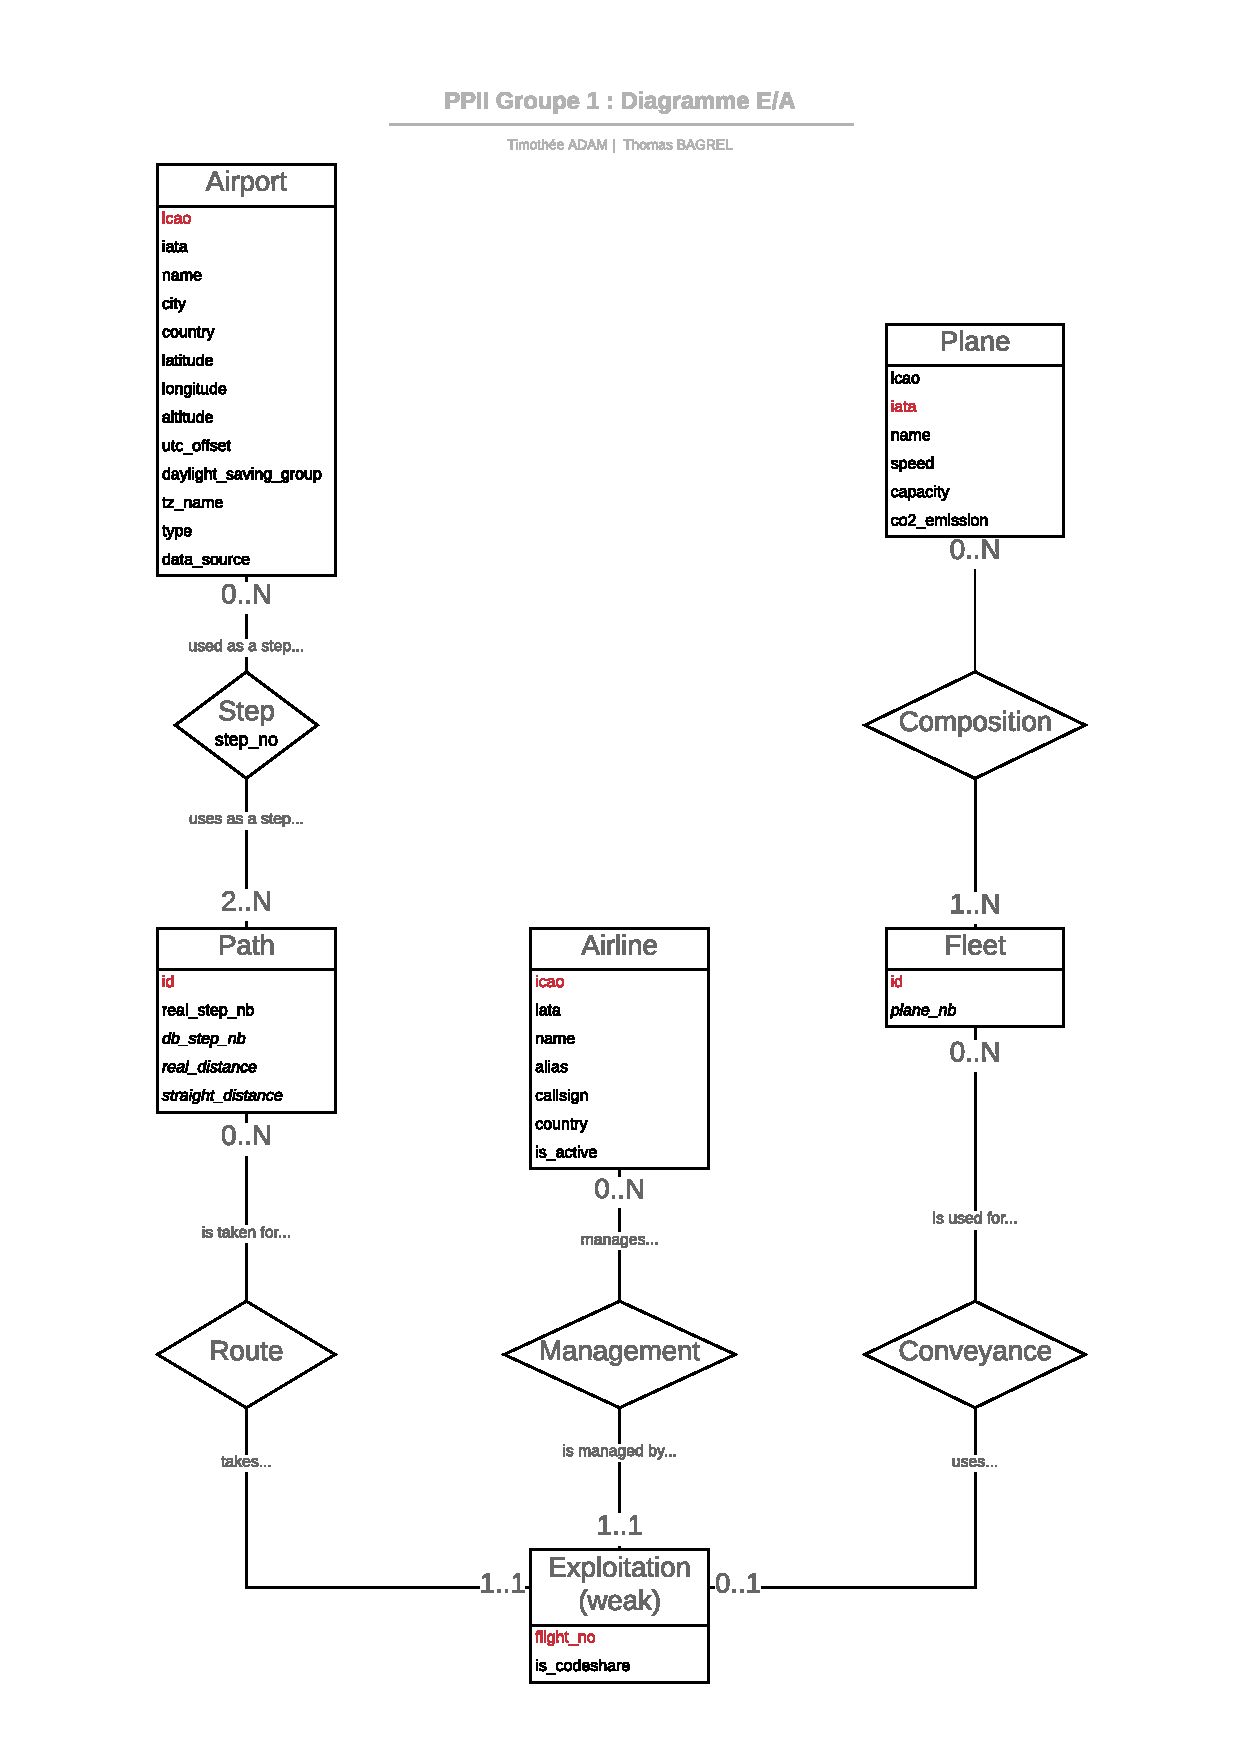
\includepdf[pages=-]{resources/e_a.pdf}
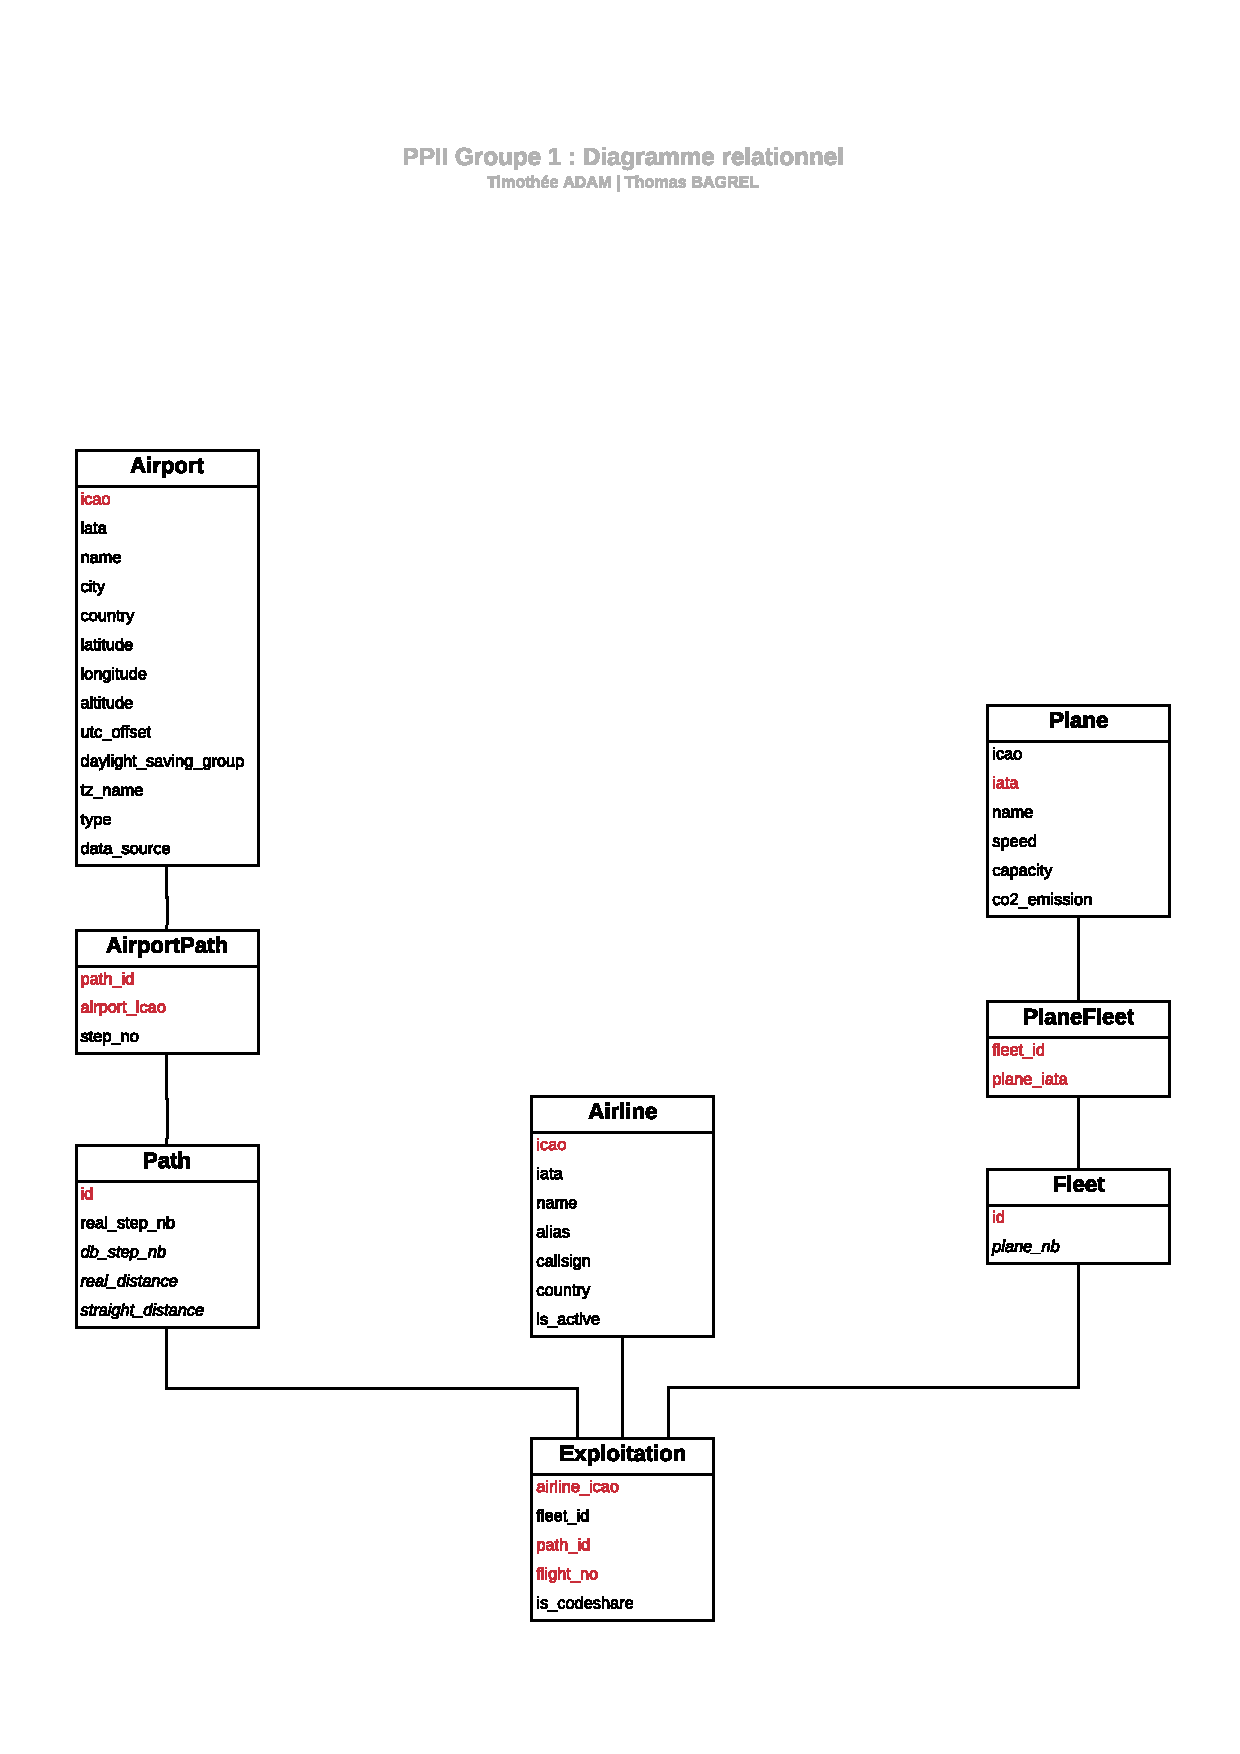
\includepdf[pages=-]{resources/schema_relationnel.pdf}
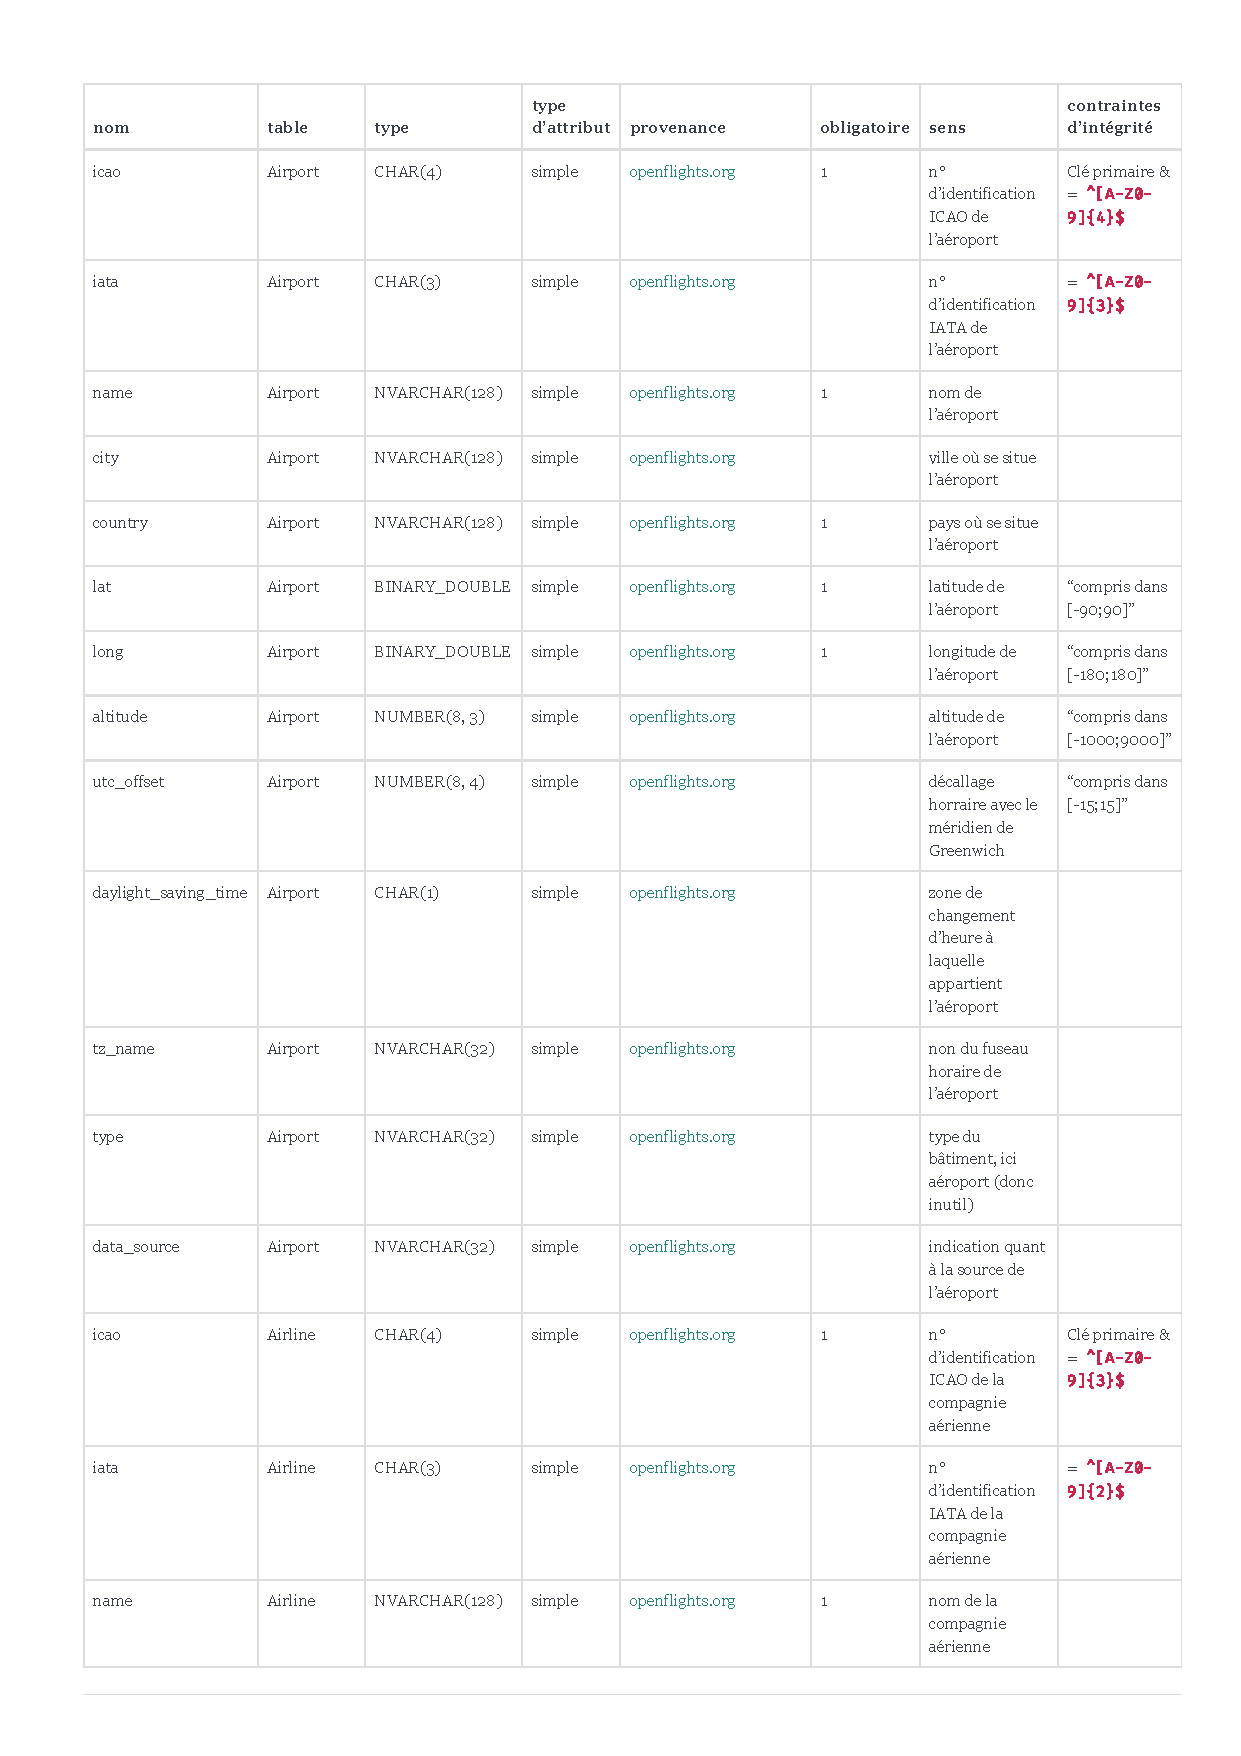
\includepdf[pages=-]{resources/doc_champs.pdf}


\end{document}
